\section{Problem 1}
\subsection{1a}

\lstinputlisting{p1a.py}

Here we test our rng as we did in the first handout. The random seed is $0$. 
\begin{figure}[h!]
    \centering
    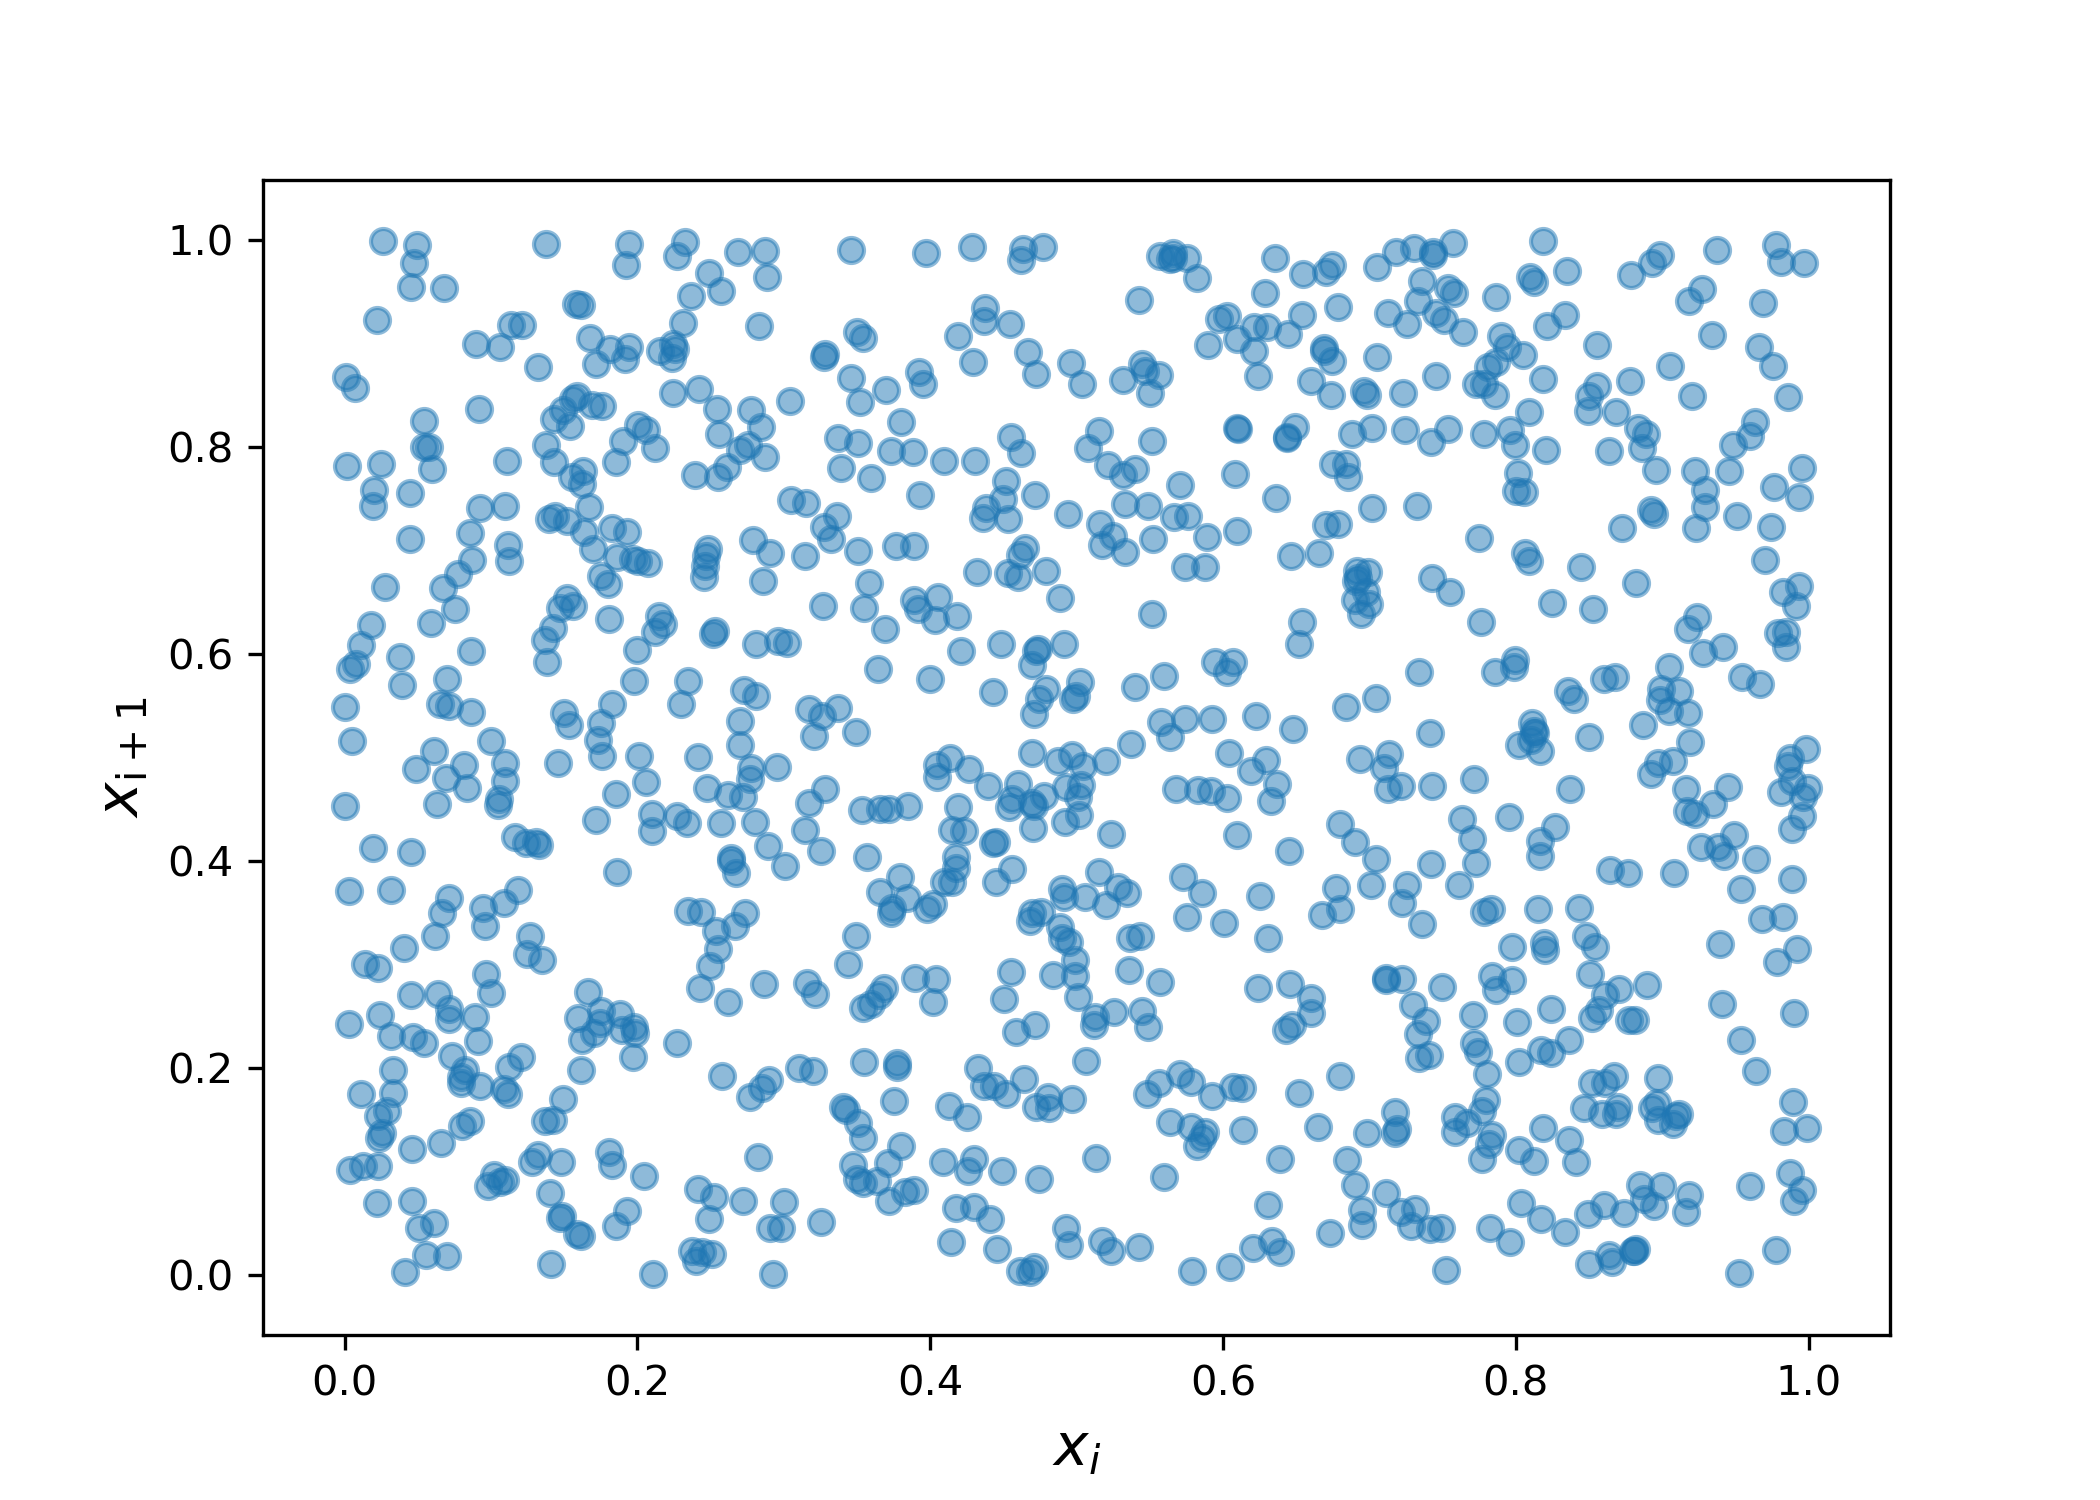
\includegraphics[width=0.9\linewidth]{./plots/x_x_1.png}
    \caption{$x$ vs. $x_{i+1}$ for the random number generator.}
    \label{plt1}
\end{figure}
Looking at the $i$ versus the $i+1$ components of our rng, there appears
to be little correlation between the numbers, which is a good sign. In
\autoref{plt2} we see the values that each number has in the array of 
$1000$ random numbers. It is between $0$ and $1$, also a good sign.
\begin{figure}[h!]
    \centering
    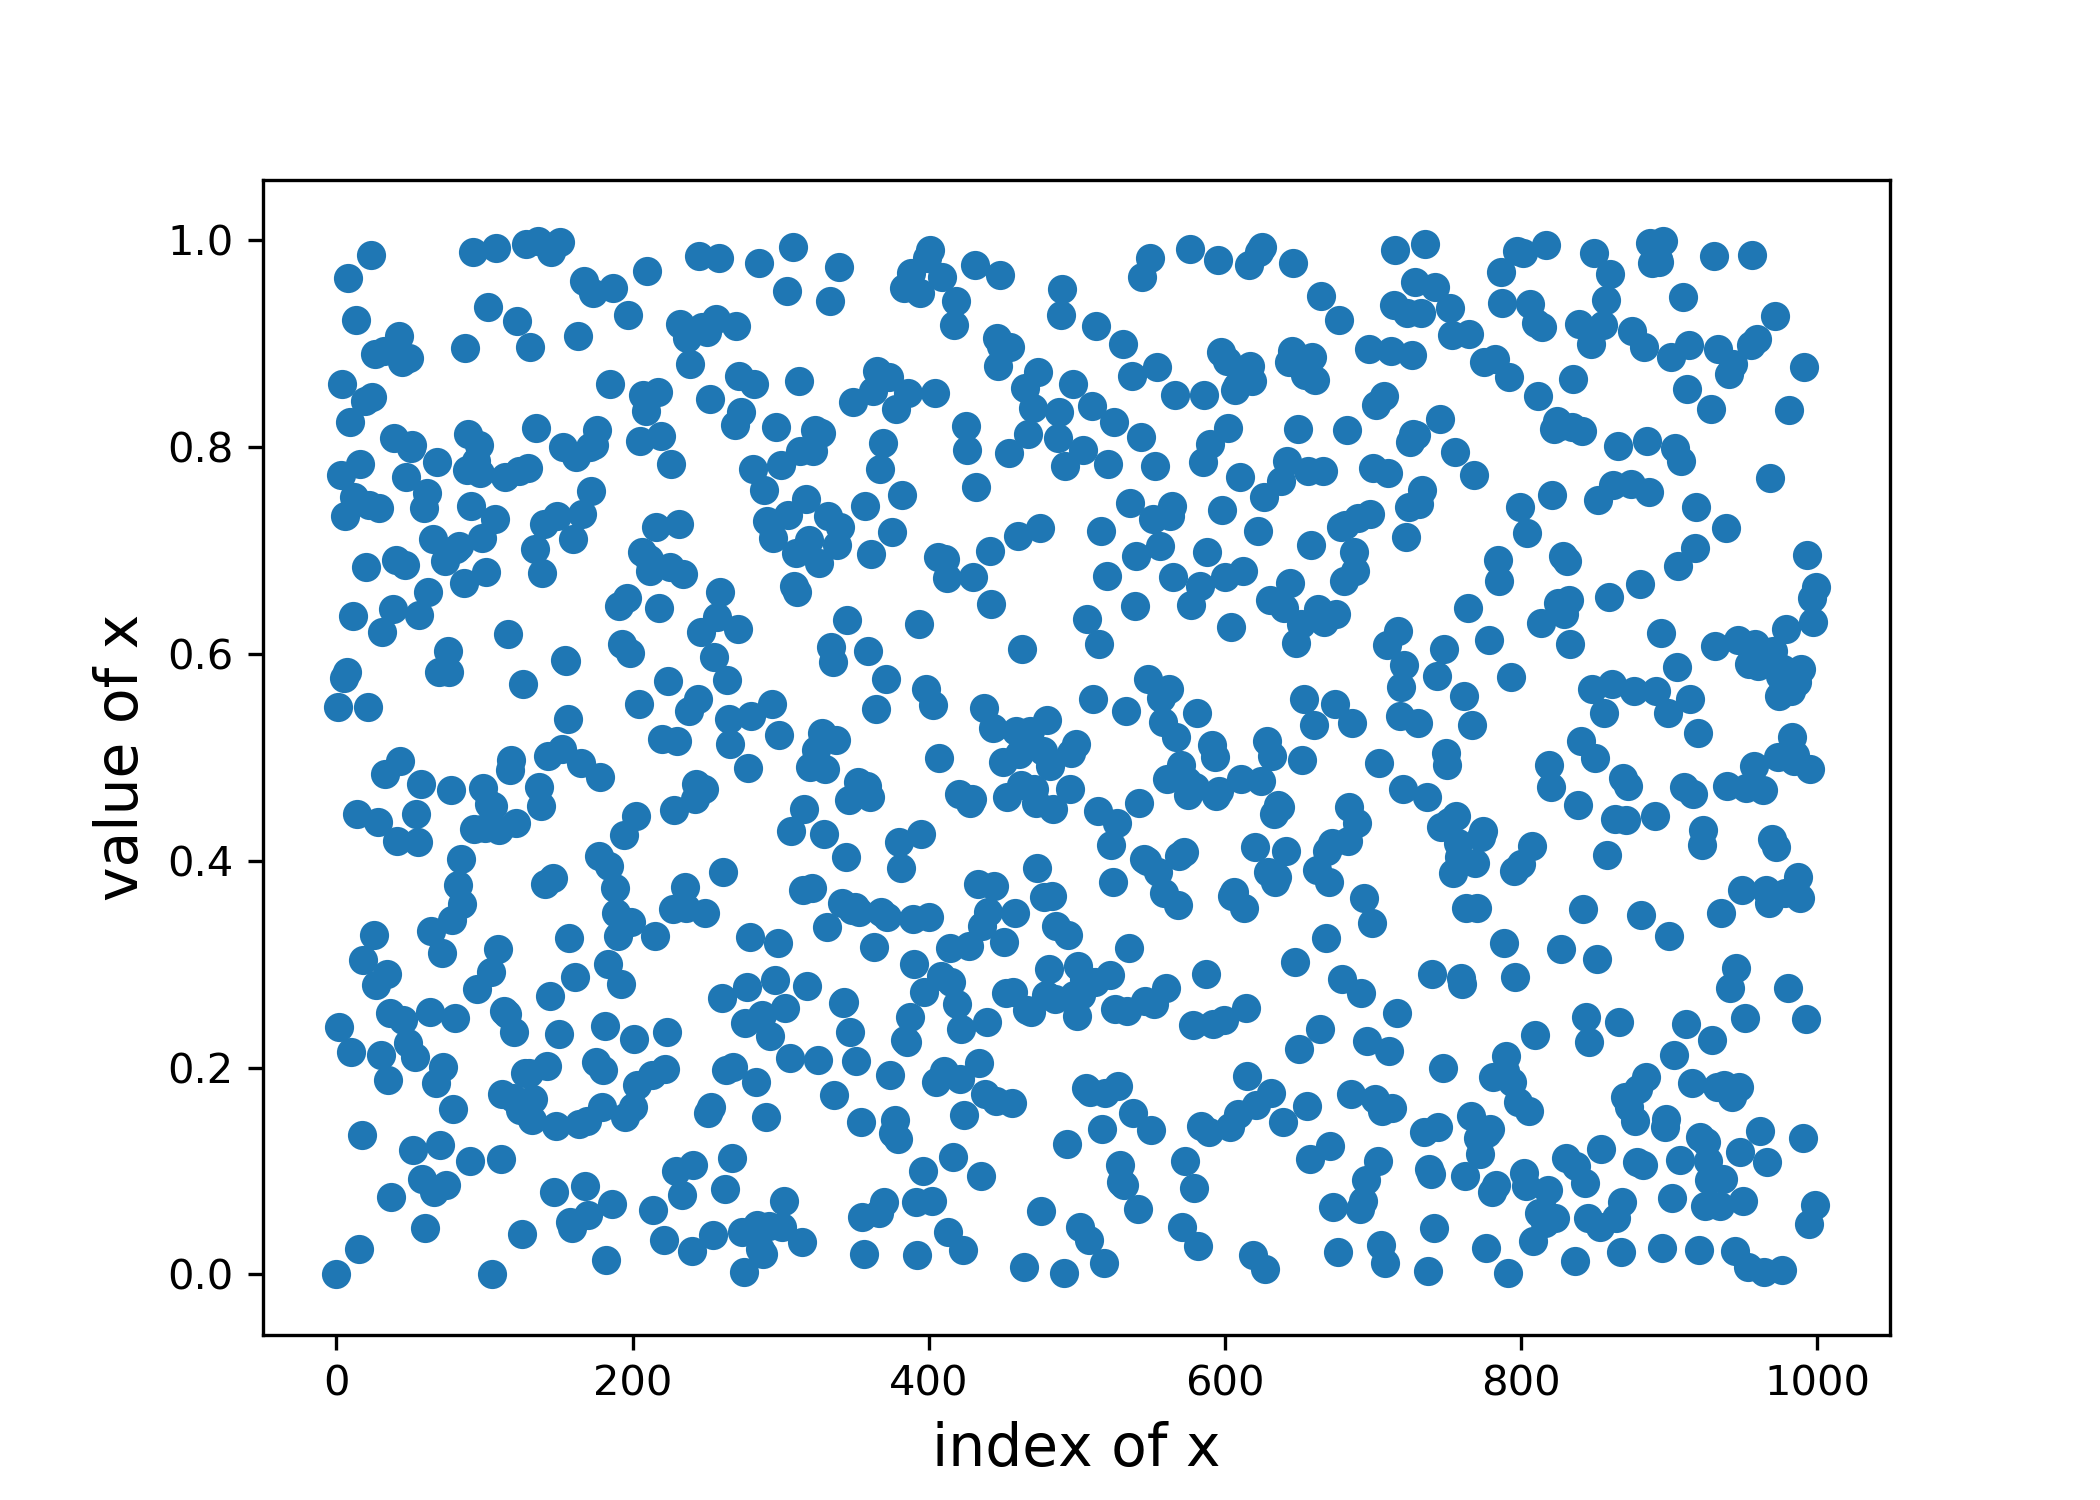
\includegraphics[width=0.9\linewidth]{./plots/xval_xind.png}
    \caption{The value of $x$ at a given index.}
    \label{plt2}
\end{figure}
However, in \autoref{plt3} it is clear something is wrong with the rng.
\begin{figure}[h!]
    \centering
    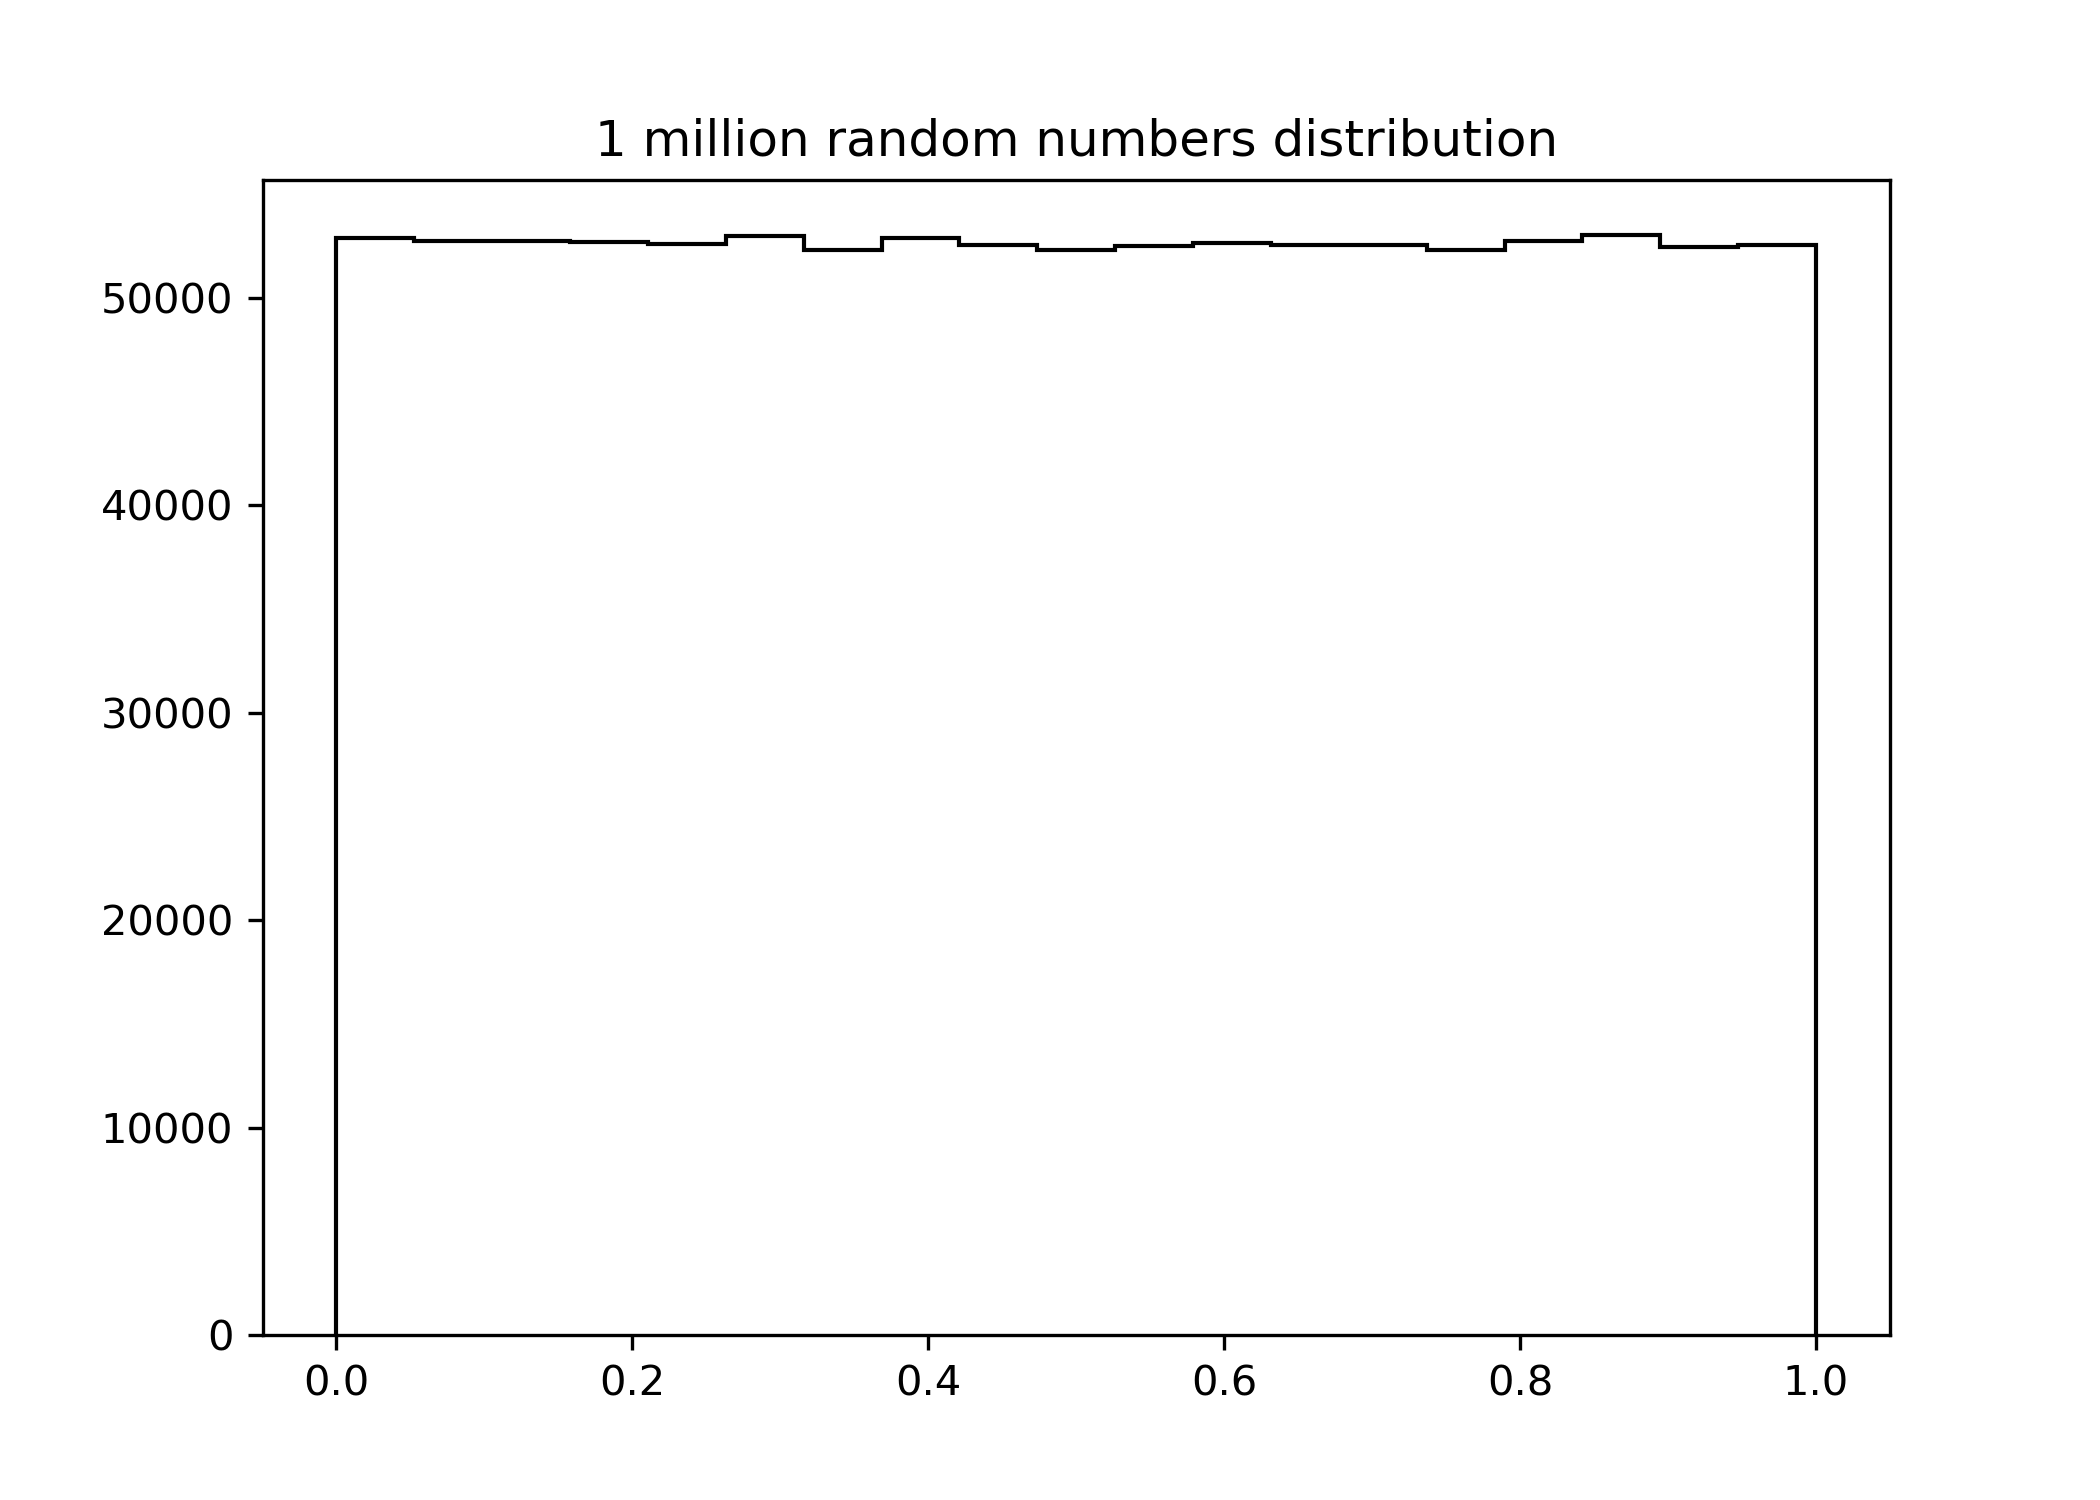
\includegraphics[width=0.9\linewidth]{./plots/1mil_hist.png}
    \caption{$1$ million random numbers plotted.}
    \label{plt3}
\end{figure}
As is plainly seen, the numbers in the random generator nearly all go above 
$5 \times 10^4$, which is not what we would expect from the rng. I am not
sure what the issue is. I attempted to cast all of the values as \texttt{ints}
but I was getting runtime errors in the $XOR$ bit-shift. The variance appears
to be fine, so I left it as is.

